\chapter{Theory}
%aj instead of theory I would suggest to name it background 
This chapter will presents theoretic concepts that help understand the methodologies used during the course of this project. First, the reader will be presented with fundamental concepts related autonomous mobile robotics. Then, theory about robotic manipulation and tag based machine vision will be explained. Finally, ROS2 is explained, as this is a vital part of the project.
% related to unmanned ground vehicle (UGV) for the application of warehouse automation. write in the verybeginning about the building block for this application - perception, autonomous navigation with collission detection and  avoidance, object detection and localization, robotic manipulation for pick and place. Then each of these becomes a section

% aj - presents. Not is future but in simple present tense. something like this
% This chapter presents the ovelying thoery behind the autonomous warehous functionalities namely ... a,b,c .. in chapter 1. Starting with the fundamental conpept of use of unmanned ground vehicle (UGV) for warehouse automation, then we describe the autonomous navigation ......Finally we intergrate individual functionalities to achieve warehouse automation.

\section{Robotic Concepts}
This thesis is focused around a mobile robotic platform with a mounted robotic manipulator. Both mobile robotics and manipulator robotics share some fundamental concepts that forms the basis of robotics. This section will touch onto some of these concepts to give the reader a level of understanding of robotics needed to better understand the methodologies in the thesis. More in depth description of these concepts and may more, can be found in \cite{LynchKevin2017Mr:m}.

A robot consists of rigid bodies, called links, connected together through joints. The links can be arranged in whichever configurations that suits the needs of the designer. For example, a serial configuration could form the familiar manipulator arm, or a parallel configuration could form a mobile robot like the differential drive robot discussed in section \ref{sec:T:AN:MRD:DifferentialDriveRobots}. Robotic joints are often, but not limited to, revolute joints. These joints are commonly driven by actuators such as electric motors.

\subsection{Kinematics}
Kinematics is the most basic study of how mechanical systems behave\cite{SiegwartRoland2011Itam}. In kinematics, the motion of a mechanical system is studied from a purely geometric point of view, meaning that forces and masses are neglected. In robotics, kinematics is fundamental for robotic control. For a robotic system to move through the environment, it need knowledge about how  its links are put together and how they move relative to each other. Kinematics is largely divided into forward and inverse kinematics. Forward kinematics studies the way a mechanical system reacts to position, velocity or acceleration inputs in it's joints. For a robotic manipulator, the pose of he end-effector is solely determined by the joint positions. Inverse kinematics studies what the position of a mechanical system's joints would need to have in order to achieve a given pose in one of it's rigid bodies.



\section{Autonomous Navigation}
% aj make it navigation, as you have a section - SLAM later that combines perception and this section
As pointed out in section \ref{sec:I:AutonomousNavigation}, for a mobile robot to be able to do autonomous navigation, four building blocks has to be fulfilled, or rather, four problems has to be solved. This section describes methods used to solve these problems in mobile robotics.

\subsection{Mobile Robot Design}
A mobile robot is designed to be able to move around in the environment. The design of the robot therefore needs to be centred around the design requirement that the robot needs an efficient way of traversing it's intended environment in a predictable manner. Predictable is important as the robotic system needs to be able to estimate it's movement. This section will introduce the reader to some common mechanisms of locomotion and a few mobile robotic designs.

\subsubsection{Locomotion}
The mechanisms that traverse the robot through the environment, is referred to as locomotion. Close to all mechanisms of locomotion are heavily inspired from nature. Examples of such locomotion mechanisms are walking, sliding, jumping, swimming and flying. However, there is one type of locomotion invented by humans that is also extremely energy efficient on hard surfaces; the powered wheel. Legged locomotion gives the benefit of adaptability and manoeuvrability in rough terrain. However, legged locomotion suffer from power inefficiency and high complexity. Wheeled locomotion is therefore by far the most popular type of locomotion in mobile robotics\cite{SiegwartRoland2011Itam}.

\subsubsection{Differential Drive Robots}\label{sec:T:AN:MRD:DifferentialDriveRobots}
Differential drive mobile robots refers to a wheeled robotic system made up of a rigid body with two driven wheels. Figure \ref{fig:differentialDrive} illustrates different types of differential drive robotic movement systems. The common denominator for all three of the robotic systems in figure \ref{fig:differentialDrive}, is that they all rely on two driven wheels.

\begin{figure}[htp]
  \centering
  \includesvg[width = 0.7\textwidth]{Figures/DifferentialDrive.drawio.svg}
  \caption{Illustration of different differential drive robotic designs. \textbf{1:} Two independently driven wheels in the rear/front, one unpowered omnidirectional wheel in the front/rear. \textbf{2:} Two-wheel centered differential drive with a third point of contact. \textbf{3:} Two-wheel differential drive with the center of mass (COM) below the axle. Figure inspired from \cite{SiegwartRoland2011Itam}.}
  \label{fig:differentialDrive}
\end{figure}

% Inspired by \cite{SiegwartRoland2011Itam}, the robot is modelled as a rigid body on wheels, interacting with a horizontal plane. The robot has a total of three DOFs, two for position, and one orientation along the orthogonal axis of the plane. Figure \ref{fig:PositionalRepresentation} illustrates how the robot is modelled and how the pose of the robot is specified on the plane. The axes $X_I$ and $Y_I$ represents a global reference frame on the plane with its origin at $O:{X_I, Y_X}$. A point P defined on the robot's chassis to act as a position reference point. Using the point P as origin, the axes $X_R$ and $Y:_R$ represents the robot's local reference frame. 

% \begin{figure}[htp]
%   \centering
%   \includesvg[width = 0.7\textwidth]{Figures/figPositionalRepresentation.drawio.svg}
%   \caption{Illustration of the local robot reference frame, $P:{X_R, Y_R}$, relative to the global reference frame, $O:{X_I, Y_I}$. The pose of the robot is given as $\zeta_I$ where $x$ and $y$ denotes position and $\theta$ denotes angular rotation of local frame relative to global frame. Figure inspired from \cite{SiegwartRoland2011Itam}.}
%   \label{fig:PositionalRepresentation}
% \end{figure}

% Looking at figure \ref{fig:PositionalRepresentation}, the position of $P$ is given as $P=(x,y)$ and the angle between the global and local reference frame is given as $\theta$. The pose of the robot becomes $\zeta_I$, where the subscript $I$ specifies that the pose is given relative to the global reference frame. Definition of $\zeta_I$ is given in eq. \ref{eq:posRep}.

% \begin{equation}
%     \label{eq:posRep}
%     \zeta_I &= \begin{bmatrix}
%                 x \\
%                 y \\
%                 \theta
%                 \end{bmatrix}
% \end{equation}


\subsubsection{Skidding Robots} \label{sec:T:AN:MRD:SkiddingRobots}
On a differential drive robot, the assumption is made that the driven wheels are not allowed to skid against the surface. However, there is an alternative type of robot where skidding is a part of the steering mechanism. Similarly to differential drive robots, these robots reorient themselves by spinning the wheels on each side of the robot at different speeds or in opposite directions. The difference is that these robots usually have tracks or several wheels on each side, giving it a much larger contact patch with the ground. The large contact patch gives these robots significantly improved traction in loose and rough terrain. Due to this large contact patch, the robot will usually skid when turning, hence the name. On some designs, the whole contact patch will be skidding when turning. This is the same type of locomotion that is used by military tanks\cite{SiegwartRoland2011Itam}. Figure \ref{fig:skidDrive} illustrates different skidding robot designs.

\begin{figure}[htp]
  \centering
  \includesvg[width = 0.7\textwidth]{Figures/skiddingDrive.drawio.svg}
  \caption{Illustration of different skidding robot designs. \textbf{1:} Tracked robot, \textbf{2:} Six wheeled robot, \textbf{3:} Four wheeled robot.}
  \label{fig:skidDrive}
\end{figure}
% aj change 1,2,3 to a,b,c
The main disadvantage of these skidding robots is that their turning nature makes it difficult to determine a center of rotation. In addition, the turning motion will be affected by differences in surface friction. This makes it significantly harder to determine the exact pose of the robot when turning compared to for example a normal differential drive robot. As a result, dead-reckoning is inaccurate for these robots and too aggressive turning motions could disorient the whole system. Another disadvantage is that the robot must overcome the static friction between the ground and the wheels/tracks to turn, this is highly inefficient on surfaces with high friction.

\subsection{Motion Control}\label{sec:T:AN:MotionControl}
Motion Control in mobile robotics refers to the actuation of motors to move  around the environment in a controlled manner. The control system calculates the actuation of the robotic motors based on inverse kinematics, moves the mobile robot by actuating its motors and estimates its movement based on wheel measurements and forward kinematics.


\subsection{Perception}\label{sec:T:AN:Perception}
In order to achieve autonomous navigation, it is essential for a robotic system to acquire knowledge of itself and its surroundings. This section gives a short introduction to a selection of different sensors that could be used to build a robotic system.

\subsubsection{Laser Range Finder}
Laser Range Finders, often known as Light Detection and Ranging (LiDAR) sensors, are sensors that utilise light to measure the distance from the sensor to an obstacle. Two different working principles are discussed in the following paragraphs; direct time-of-flight and indirect time-of-flight.

Direct time-of-flight based LiDARs bases itself on directly measuring the round-trip time of a light pulse. The sensor transmits a light pulse and then measures the time it takes before this light pulse returns after bouncing off an obstacle. The distance, $d[m]$, between the sensor and the obstacle can then be calculated based on the speed of light $c=3X10^8[m/s]$, and the delta time, $\Delta t[s]$. Equation \ref{eq:TOF} describes the relationship between these variables.

\begin{equation}\label{eq:TOF}
d = \frac{c \cdot \Delta t}{2}
\end{equation}

The measurement is divided by two as the light travels the distance twice, to the obstacle and back. One disadvantage of this principle, at least for laser range finders, is that it places high requirements on the electronics of the sensors. As an example, if an obstacle is placed 1[m] away from the sensor, the round-trip time of the light pulse would be $\Delta t=6.667X10^{-9}[s]$. Accounting for the Nyquist–Shannon sampling theorem, which states that a measurement needs to be more than twice the frequency of the measured signal in order to be sufficient. Since $f_{\Delta t}=150MHz$, the sampling frequency would have to be more than $B=300MHz$ in order to detect that signal. 

Indirect time-of-flight sensors rely on emitting a modulated light wave and then looking at the phase shift of the returning measurement. The phase shift is directly related to the distance between the sensor and the object. Based on the phase shift $\phi[rad]$, the speed of light $c=3X10^8[m/s]$ and the modulation frequency $f_m[Hz]$, the distance between the sensor and the object can be calculated as seen in equation \ref{eq:iTOF}. In this case, the distance is also divided by two as the light travels twice the distance.

\begin{equation}\label{eq:iTOF}
d = \frac{c \cdot \phi}{2\pi \cdot 2 \cdot f_m}
\end{equation}

Since the phase shift is measured in the frequency domain, several cycles of the modulated light pulse, are required to complete one measurement. This might prove impractical for some applications.

Using one of several time-of-flight principles, for example direct time-of-flight, a two-dimensional LiDAR sensor can be made by rotating the sensor and mapping the measurements to the rotation. This can also be expanded to three dimensions by rotating a vertical array of sensors, creating a rotating vertical sensor beam.

% aj add camera, radar, thermal camera


\subsection{Localisation}\label{sec:T:AN:Localisation}
%aj i would suggest make the title simultaneous localization and mapping. Then odometry, ... kalman filter becomes the part of it
Robot localisation involves the robot building a map of the robot's environment, and determining its position relative to this map\cite{SiegwartRoland2011Itam}.  To achieve successful localisation, a combination of different localisation techniques is often used. As an example, a mobile robot could combine odometry with IMU and LiDAR measurements to determine its position. The following paragraphs discuss these localisation implementations.

% \subsubsection{Wheel Encoders}
% To estimate chassis travel, an autonomous robot utilises rotational encoders to measure wheel movement. A rotational encoder may be based on one of many functional principles, but the common denominator for all rotational encoders are that they measure  rotational displacement. 
% % ØØ ---------- Might not need this?? --------

\subsubsection{Odometry}
Odometry in mobile robotics refers to the use of wheel sensors and forward kinematics to estimate the position of the robot over time. Wheel encoders are usually relative, meaning that they don't provide an absolute measurement on the displacement of the wheels. As a result, wheel odometry relies on integrating the wheel movement over time and then using this to estimate the robot's position relative to a starting position. The accuracy of this pose estimation method highly dependant on the mobile robot's design and the wheel sensor accuracy. Because of the integrating, the measurement errors accumulate over time, making odometry drift over time.

\subsubsection{Inertial Measurement Unit}
An Inertial Measurement Unit(IMU) is a device that combines accelerometers, gyroscopes and magnetometers to measure the acceleration, angular movement and orientation of a body. IMUs are often used to help determine the localisation of vehicles, and robots. Using IMU measurements, the movement of an object can be estimated by integration time, as with odometry. This is called dead reckoning and similarly to odometry, the measurement errors is integrated over time resulting in drift.
% Do i need sources for this or is it fine?


\subsubsection{Kalman Filter \& Extended Kalman Filter}
An Extended Kalman Filter(EKF) is often used in robotics to fuse several sensor measurements and estimations to one optimal estimate. This way, no one measurement has to be chosen and no measurements has to be discarded. To understand what an EKF is, one must first have an understanding about traditional Kalman Filters. A Kalman Filter uses a Gaussian distribution to represent the belief of the robots location. A Gaussian only has two parameters, its mean $\mu$, an covariance $\Sigma$. As there are only two parameters that are updated during each prediction, this results in a very efficient algorithm. However, it also means that the filter needs to have an initial belief that is close to it's actual position in order to be effective. It also has no way of recovering it's position if it gets lost. Figure \ref{fig:kalmanFilter} is an illustration from \cite{SiegwartRoland2011Itam} that demonstrates Kalman Filter localisation working principle. The robot is represented in a one-dimensional environment and it's positioning belief, $bel(x)$, is represented as a Gaussian distribution. From figure \ref{fig:kalmanFilter} \textit{(a)}, the robots initial is represented as a fairly confident Gaussian. The robot then moves, and in figure \ref{fig:kalmanFilter} \textit{(b)} the robot has estimated its position using it's wheel odometry. Since odometry accumulates measurement errors, it's belief is now represented as a less confident Gaussian. Next, the robot uses its perception system and sees that it is near the second pillar. This results in a posterior probability $p(z_t | x_t,M)$ of the observation represented as a Gaussian in figure \ref{fig:kalmanFilter} \textit{(c)}. The posterior observation is then fused with the robots belief after moving (fig. \ref{fig:kalmanFilter}\textit{(b)} and represented as $bel(x)$ in figure \ref{fig:monteCarloLocalisation}\textit{(c)}. It can be seen that this belief is more confident(narrower) than the two Gaussians it is comprised of. This makes sense since the two independent measurements agree and that would result in a more certain estimate. In the last step, seen in figure \ref{fig:kalmanFilter}\textit{(d)}, the robot has moved again and convolved its odometry with the previous belief. Because of the uncertainty of the odometry, the resulting belief is less confident.

\begin{figure}[htp]
  \centering
  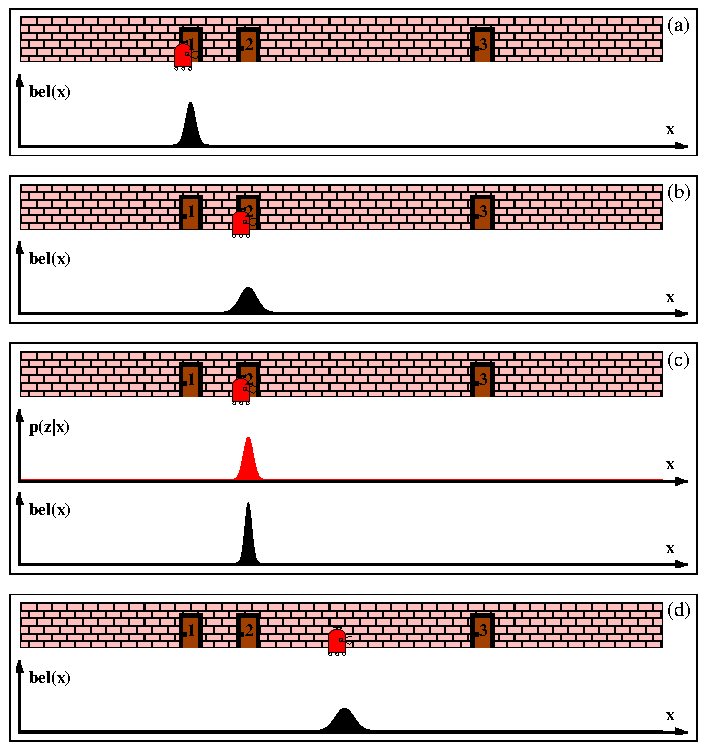
\includegraphics[width = 0.7\textwidth]{Figures/figKalmanFilter.pdf}
  \caption{Kalman Filter demonstration in a one-dimensional environment. Each figure, \textit{(a), (b), (c), (d)} represents a robot and it's positional belief $bel(x)$ as a Gaussian distribution. \textbf{(a):} The robots initial belief. \textbf{(b):} The robots belief after moving and convolving odometry with initial belief. \textbf{(C):} The robot observed the second pillar and gained a posterior probability $p(z|x,M)$. Fusing this with the belief from \textbf{(b)} results in a narrower belief $bel(x)$. \textbf{(d)} Robots belief after moving again and convolving the odometry with the previous belief. Figure from \cite{ThrunSebastian2005Pr}}
  \label{fig:kalmanFilter}
\end{figure}

Kalman Filters assume the system to be linear and with white Gaussian noise. However, most robotic applications are nonlinear. The algorithm therefore has to linearise the system before applying the Kalman Filter \cite{SiegwartRoland2011Itam}. This extension to the original Kalman Filter gives it the name EKF. Linearisation is a simplification of what could otherwise be a complex n-th order system. The result is that the EKF may only work within a certain operating range of the system and may not be helpful at all. For more info on Kalman Filters and EKFs, see \cite{SiegwartRoland2011Itam} or \cite{ThrunSebastian2005Pr}.

\subsubsection{Monte Carlo Localisation}
EKFs are computationally efficient and a great tool to improve probabilistic localisation. However, an EKF based localisation would not be able to do \textit{global localisation} (initial position is unknown, \cite{SiegwartRoland2011Itam}, \cite{ThrunSebastian2005Pr}) or solve the \textit{kidnapped robot problem} (robot gets kidnapped and moved to another location \cite{SiegwartRoland2011Itam} \cite{ThrunSebastian2005Pr}). In this case, a particle based localisation method like Monte Carlo Localisation(MCL) has proven to be successful. Figure \ref{fig:monteCarloLocalisation} is used to better explain how MCL works. The figure and description is adapted from \cite{ThrunSebastian2005Pr}. The figure illustrates a robot in a one-dimensional corridor. The belief $bel(x)$ is represented as pose particles with a height corresponding to their importance factor, hence the particle filter definition. In figure \ref{fig:monteCarloLocalisation}\textit{(a)} the global uncertainty is illustrated through a set of pose particles drawn at random and uniformly over the entire pose space. The robot could be anywhere in the corridor. Then, the robot senses the door and gives a posterior probability $p(z|x)$. MCL gives a importance factor to each particle from the initial particle sampling. The resulting belief$b(x)$ along with $p(z|x)$ can be seen in figure \ref{fig:monteCarloLocalisation}\textit{(b)}. In figure \ref{fig:monteCarloLocalisation}\textit{(c)} the robot has re-sampled the particle set and implemented its movement. It can be seen that the particles are now more densely populated around the most likely poses, but with uniform importance factors. The robot then senses another door and gives the posterior probability $p(z|x)$ again. Looking at figure \ref{fig:monteCarloLocalisation}, it is worth noticing that the posterior probability from \textit{(b)} and \textit{(d)} is equal, as the door sensor won't know the difference between each door. MCL again gives importance factors to each particle, as seen in the belief $bel(x)$ in figure \ref{fig:monteCarloLocalisation}\textit{(d)}. This time, most of the total particle mass is centred around the second door, which is also the robots position according to the illustration. In figure \ref{fig:monteCarloLocalisation}\textit{(e)}, the robot has moved and re-sampled the pose particles, which is centred around the most likely pose of the robot.

\begin{figure}[htp]
  \centering
  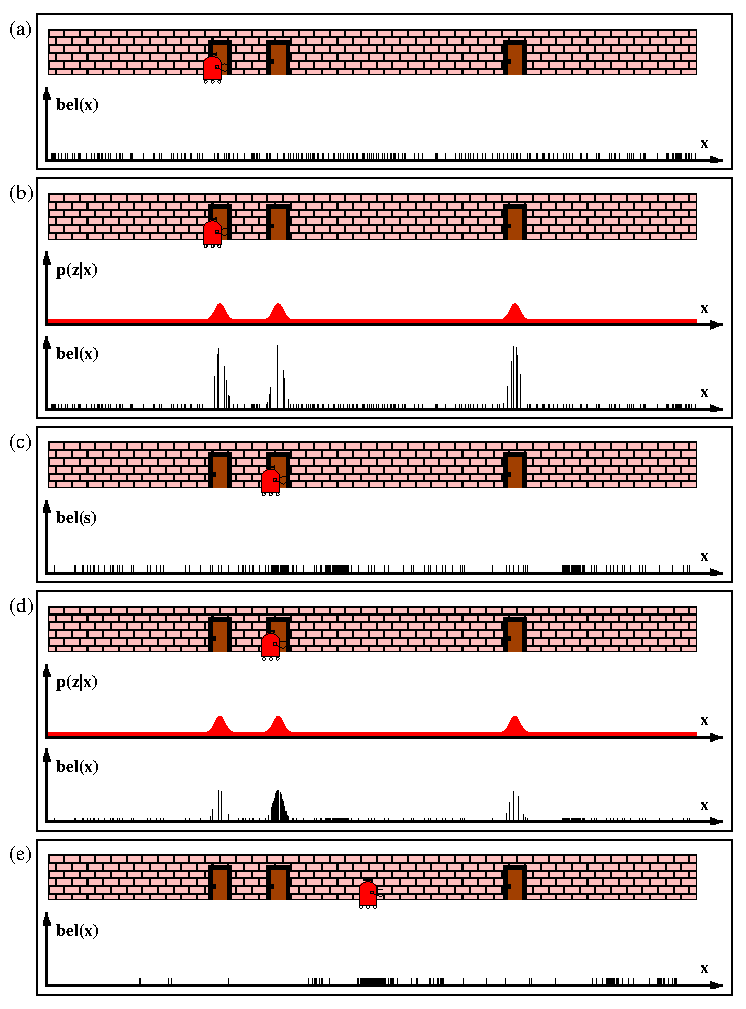
\includegraphics[width = 0.7\textwidth]{Figures/figMCL.pdf}
  \caption{Monte Carlo Localisation a one-dimensional environment. Figure from \cite{ThrunSebastian2005Pr}.}
  \label{fig:monteCarloLocalisation}
\end{figure}

\subsubsection{KLD-Sampling Monte Carlo Localisation}
Plain MCL use particle sample sets of fixed size. At an early stage of localisation, when the robot does not know where it is, the sample set needs to be large to avoid divergence. However, when the location of the robot is fairly confident or known, it is computationally inefficient to have an unnecessarily large particle set. A variant of MCL, called KLD-sampling, adapts the number of particles based on Kullback-Leibler divergence(KLD). Kullback-Leibler divergence is a measure of the difference between two probability distributions. KLD-sampling use KLD to create a measure for the difference between the true posterior belief provided by measurements, and the sample based approximation of this belief. To read more about this localisation method, pleas refer to the source \cite{ThrunSebastian2005Pr}.

\subsection{Simultaneous Localisation and Mapping} \label{sec:T:AN:L:SLAM}
Both EKF-localisation and MCL assumes that it is given a map of the environment. Although there could be a pre-made map that fits the application, this is often not the case. The robot therefore has to do the mapping and localisation at the same time. This problem is called the Simultaneous Localisation and Mapping(SLAM) problem. One of the more popular solutions to the SLAM problem is by the use of pose graphs \cite{Konolige2010}. A pose graph is a sparse graph of nodes with constraints between them. The nodes in the graph are different robot poses and features of the map. The constraints represents the relative relation between the robot poses and also between robot poses and features of the map. It is important to specify that the constraints between the poses are non-rigid. The pose graph can therefore be interpreted as an elastic net of poses. The solution is then to find the state where this net has the minimum amount of energy \cite{SiegwartRoland2011Itam}. Figure \ref{fig:poseGraph} illustrates how a pose graph is built from different robot and map feature poses as a robot moves through an environment. As the map becomes larger, the size of the pose graph also increases, which in turn results in an increased computational effort required for optimisation. A method of pose graph optimisation that has proven efficient, is Sparse Pose Adjustment (SPA)\cite{Konolige2010}. A  map can be constructed as for example an occupancy grid map (described in \cite{ThrunSebastian2005Pr}) when the pose graph is constructed and optimised. \cite{SiegwartRoland2011Itam} and \cite{ThrunSebastian2005Pr} provides more information on SLAM.

\begin{figure}[htp]
  \centering
  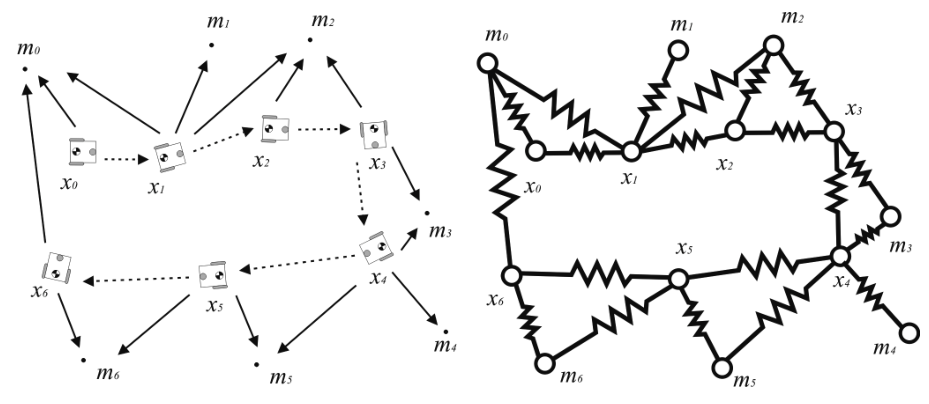
\includegraphics[width = 0.9\textwidth]{Figures/figposeGraph.pdf}
  \caption{Demonstration of pose graph. The illustration demonstrates how robot and map feature poses are presented as nodes with flexible constraints between them to generate a pose graph. Robot poses are denoted as $x_i$ and map feature poses are denoted as $m_n$. Figure from \cite{SiegwartRoland2011Itam}.}
  \label{fig:poseGraph}
\end{figure}


\subsection{Path Planning}\label{T:AN:PathPlaninng}
Path planning involves finding a trajectory that the robot can follow to reach it's goal \cite{SiegwartRoland2011Itam}. Path planning in mobile robotics draws from the extensive research done in this area for robotic manipulators \cite{SiegwartRoland2011Itam}. However, path planning for mobile robots is usually far less complex than that of manipulators due to the reduced degrees of freedom and the fact that manipulators often operate in such high speeds that the dynamics of the system has to be taken into account\cite{SiegwartRoland2011Itam}. A robotic manipulator typically has five or six degrees of freedom, whereas a mobile robot typically operates in a plane with three degrees of freedom. There are numerous different path planning algorithms available, two of the more popular path planning algorithms for use in mobile robotics is Djikstra's Algorithm and A*. When talking about path planning for mobile robotics, a \textit{node} represents a position, often in a grid-based map and an \textit{edge} represent the path from one node to a neighbour node. 

\subsubsection{Djikstra's Algorithm}\label{T:AN:PP:DjikstrasAlgotihm}
Djikstra's algorithm is a planning algorithm published by E. W. Djikstra in 1959\cite{DijkstraE.W1959Anot}. The algorithm presents a way to find the shortest path from a starting point $P_s$ to a goal $P_g$. This is done by giving a cost to the path it finds from $P_s$ to each node in the map, it will keep the paths with the lowest cost and keep searching until it has found the lowest cost path from $P_S$ to all nodes in the map. For each iteration, the algorithm will explore the unexplored node with the lowest calculated cost. The cost is usually based on distance or time taken to traverse the edge. In mobile robotics, the algorithm is often computed from the $P_g$, meaning that it will find the shortest path to any $P_s$ in the map. Thus, the robot is able to plan the best path to the goal based on it's current position without running the planning algorithm again \cite{SiegwartRoland2011Itam}. For example, if the robot is moving towards the goal and needs to take evasive actions because of some moving obstacle in it's trajectory. Time complexity for this algorithm is noted as $O(n\log(n)+m)$ where $n$ is the number of nodes and $m$ is the number of edges\cite{SiegwartRoland2011Itam}. See \cite{DijkstraE.W1959Anot} and \cite{SiegwartRoland2011Itam} for more information about the algorithm. 

\subsubsection{A* Algorithm}\label{T:AN:PP:DjikstrasPlanning}
The A* algorithm is similar to Djikstra's algorithm in that it will give the edges between the nodes a cost. However A* also carries a heuristic which estimates the distance from explored nodes to the goal, $P_g$. For mobile robotics, this heuristic is often calculated as the distance between any cell and the goal cell, $p_g$ in the absence of obstacles (straight distance) \cite{SiegwartRoland2011Itam}. This way, the algorithm will usually explore nodes located in the direction towards the goal before expanding in any other direction. Because of this, the algorithm is often much faster than for example Djikstra's, but it is not guaranteed that the lowest cost path is found. The time complexity of this algorithm is also largely dependent on the weighting of the heuristic and the geometry of the map. See \cite{SiegwartRoland2011Itam} for a more in-depth explanation of the algorithm.

% \subsection{Obstacle Avoidance} \label{T:AN:PP:ObstacleAvoidance}
% Obstacle avoidance refers to the act of avoiding obstacles that are detected by the robot's sensors in order to avoid collision. As an example, if a pedestrian is standing in the robot's trajectory, then the local planner divert the robot so that it moves around the pedestrian instead of running into it. After the evasive action has taken place, the robot should have adjusted it's trajectory so that it can keep following it to reach it's goal. A popular method for obstacle avoidance is the dynamic window approach. This approach takes 

% ------------ØØ - AJ, Do i need to talk about obstacle avoidance/local path planning?  --------------------------------------
% \section{Pick and Place}
% In the context of this thesis, pick and place refers to the complete pipeline of searching for and detecting an object using machine vision, picking it using a robotic manipulator, and placing the object on another location. This section will introduce some different methods for object detection and mention some core concepts on robotic manipulation that is necessary to understand when delving into the work of this thesis.

% \subsection{Machine Vision}
% Machine vision is a 
\section{Object Detection \& Pose Estimation}\label{sec:T:ObjectDetection}
Object detection in the context of this thesis refers to the act of detecting an object in the environment using machine vision. Pose estimation refers to finding the 6-DOF pose of the detected object, that is $x,y,z,\rho, \theta, \phi$ There are a multitude of different methods that could solve this problem. 

\subsection{Machine Learning Based Object Detection \& Pose Estimation}
Machine learning based approaches for object detection and 6-DOF pose estimation could provide a robust
% ----------ØØ - AJ, Do you have a better naming convention for orientation? -------------

\subsubsection{Tag Based Object Detection }\label{sec:T:OD:TagBasedObjectDetection}


% \section{Robot Operating System 2}
% Robot operating system 2 is an open source operating system for robots that is aimed at simplifying the communication between different sensors and actuators in a robotic system, and present the information from these different sensors and actuators in a standardised matter.
% % aj not needed

% \subsection{URDF}
% % aj not needed


%\section{Conclusion}
% we described the building block that forms the basis of our Thesis aimed towards warehouse automation - perception, autonomous navigation, object localization, robotic manipulation. each chapter should have an introduction mentioning what IS covered and end with conclusion mentioning what WAS covered.